\section{LITERATURE REVIEW}

Firstly, core definitions have to be established for key concepts to provide a foundational and universal understanding, followed by in-depth analysis of gamification  aspects and theories to achieve the desired results.

\begin{enumerate}
  \addtolength{\itemsep}{-0.5\baselineskip} 
  \item Gamification and Digital and Open badges.
  \item Gamification Aspects, Game Elements.
\end{enumerate}

Definitions will be drawn from existing research works and recent studies to capture historical evolution and contemporary perspectives. 
After establishing the terminology, core aspects relevant to the project will be identified - user engagement with gamified systems, motivation, and the integration of gamified systems in educational settings and web spaces. 
This will be done with the goal of exploring their role in fostering self-determination, enhancing learning outcomes, and improving user adoption. 
Finally, critical elements for the success of the browser game are to be established for achieving the goal of the project.

%
\subsection{Establishing Core Concepts}

\subsubsection{Gamification}
%
The term itself was coined by Nick Pelling in 2002, who used it to describe the use of "game-like accelerated user interface design to make electronic [ATM vending machine] transactions both enjoyable and fast" \footnote{https://nanodome.wordpress.com/2011/08/09/the-short-prehistory-of-gamification/}. 
The greater academic exploration of gamification began around the 2010s, with researchers like Deterding and others (\cite{definition}) formalizing the concept as the incorporation of game-like design elements, which aim to leverage intrinsic human motivations, into non-game contexts.
Early 2010s definitions of gamification often reflect a similar focus on game mechanics - \textcite{definition2} defines gamification as "the use of game thinking to engage people, motivate action, and promote learning".

In contrast, later definitions such as Huotari and Hamari (2017) provide a more nuanced approach to the topic, describing gamification as "a process of enhancing a service with affordances for gameful experiences in order to support users' overall value creation" (\cite{redefinition}).
This definition broadens the scope beyond individual game elements, focusing on how gamification can achieve a much more nuanced effect on people. 
And not without good reason, as recent statistics find gamification to increase engagement in online learning platforms by 90\% \footnote{https://review42.com/resources/gamification-statistics/\_gl=1*9edevd*\_gcl\_au*NTMyNzk5MTM3LjE3MjI1NDA5NTc.}, according to informal market research, leading to the understanding of why so many platforms today are proudly applying a gamified approach to education, such as Brilliant.org, Duolingo, Khan Academy and others finding great success. 
Another contrasting view is presented by Zichermann and Cunningham (2011), who argue that gamification can sometimes lead to superficial engagement if not aligned with intrinsic user motivations. 
They suggest that without a deep understanding of the target audience's needs, gamified elements might fail to produce meaningful engagement or long-term behaviour change (\cite{bookOnEngagement}). 
The critique highlights the potential pitfall of applying gamification indiscriminately and stresses the importance of aligning gamification strategies with user motivations and context. In regard to user qualities, in Figure \ref{fig:gamifiedVSnongamified} we can see a study result which found that introverted students will tend to engage with gamified systems more than extroverted students - introverted students have a higher correlation with progression and achievement within the gamified system, based on research by Smiderle et al (\cite{gamifiedChart}).\\
\begin{figure}[htbp]
 \centering
 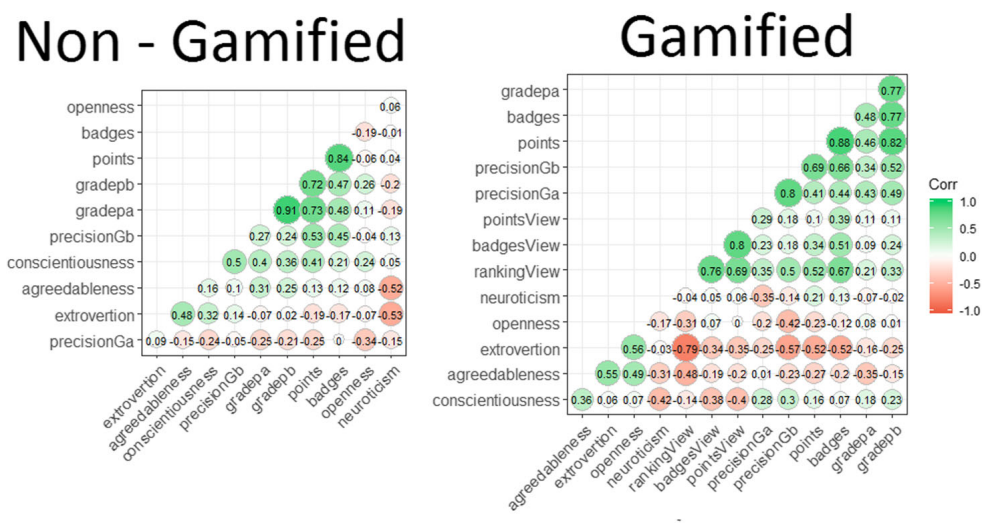
\includegraphics[width=\textwidth]{Media/chart.png}
 \caption{Correlogram for the relationship between all variables of the experiment}
 \label{fig:gamifiedVSnongamified}
 {\raggedright \small{Source: Smiderle et al., 2020}\par}
\end{figure}
Drawing from foundational definitions by Pelling (2002), Deterding et al. (2011), and Huotari and Hamari (2017), the analysis will focus on gamification as a tool to foster engagement, motivation, and learning outcomes with content or system.

In summary, gamification has proven to be a versatile and impactful strategy across various domains, supported by empirical evidence demonstrating its ability to enhance engagement, motivation, and learning performance. 
This scientific backing underscores the potential of gamification to transform user experiences and drive behaviour through the strategic application of game design principles.\\
%
\subsubsection{Digital and Open Badges}

Digital badges - visual representations of skills, achievements, or competencies earned by individuals through various learning or professional activities. 
This concept harkens back to traditional merit badges, that signify accomplishments in a tangible form, such as those awarded in organizations like the Boy Scouts. 
However, digital badges expand upon this concept by using technology for verification and credibility.

Research (\cite{GibsonBadges}) indicates that digital badges appeared in literature around 2010, which suggests a scarcity of comprehensive literature on the topic . 
The definition used for digital badges was "electronic representations of achievements or skills...", which matches the definition of traditional badges. 
It is however followed with "...including metadata that verifies the awarding body and the context of the achievement." 
This suggests that metadata is the core difference between the traditional and the digital - it contains essential information about the issuer, criteria for earning the badge, and evidence supporting the achievement. 
This transparency enhances their credibility and utility across various contexts (\cite{Bowen02012014}).

The first notable project with digital badges is considered The Mozilla Open Badges project, launched in 2011, as it created a standardized framework for their design, issuance, and verification\footnote{https://support.mozilla.org/en-US/kb/mozillas-open-badges-project}. 
This initiative allowed badges to be shared across platforms and promoted their recognition in educational and professional environments (\cite{credentialsBadges}).

Such new functionality was immediately appealing for adoption within educational contexts to more effectively and verifiably recognize informal learning, complementing traditional academic credentials. 
According to research (\cite{areBadgesUseful}), they are motivational tools that provide learners with tangible evidence of their achievements. 
Furthermore, their ability to integrate gamified elements—such as progression systems, competition and reward structures—aligns them with broader trends in educational innovation. 
Recent studies indicate that incorporating badges into online courses can lead to higher completion rates and improved learning outcomes (\cite{higherRates}).\\
{Digital Badge Characteristics}
%
\begin{figure}[htbp]
 \centering
 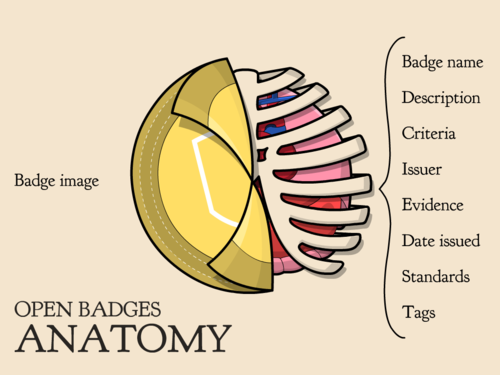
\includegraphics[width=14cm]{Media/OpenBadgeAnatomy.png}
 \caption{Open Badge Anatomy}
 \label{fig:badgeAnatomy}
 {\raggedright \small{Source: Awero team, badgecraft.eu, 2024}\par}
\end{figure}
%
\begin{enumerate}
  \addtolength{\itemsep}{-0.5\baselineskip} 
  \item Visual Symbols: Graphical representations that signify the type of achievement, skill or progress within a field. 
  This allows for easily identifiable information about the owner of the badge.
  \item Metadata-Enhanced: Each badge includes metadata that provides information about the issuer, potentially the criteria for earning the badge, as well as evidence of achievement in the form of uniquely trackable data. 
  An example anatomy is shown in Figure \ref {fig:badgeAnatomy} \footnote{https://www.badgecraft.eu/en/blog/open-badges/understand-badge-meta-data}. 
  In all cases, the badge name, description and criteria are mandatory with the rest being optional.
  This metadata ensures transparency and helps validate the badge's significance.
  \item Portable Credentials: Badges can be easily shared across platforms such as social media, professional networks like LinkedIn, and personal websites. 
  This invites for quick transferability of verifiable information. 
  Notably, since badges represent primarily informal learning, as of writing this work, they do not inherently compete with professional networks and are intended as an extracurricular display of interests or abilities rather than professional or academic prowess.
\end{enumerate}

%
Both open badges and digital badges are forms of online credentials that signify skills, achievements, or competencies. 
However, there are significant differences in their frameworks. The key areas separating the two:
\begin{enumerate}
    \addtolength{\itemsep}{-0.5\baselineskip} 
  \item {Standards.} Using the framework created by the Mozilla Open Badges Project, a set of criteria is in place regarding the creation, issuance and verification of badges. 
  According to \textcite{whatIsAnOpenBadge}, for a badge to be classified as an open badge, it must be portable, shareable, controllable, and verifiable by both the issuers and the earners. 
  This standardization is in place to ensure that open badges carry metadata that provides comprehensive information about the learning experience, including badge criteria, issuer details, and evidence of achievement. 
  In contrast, general digital badges do not necessarily follow these standards. 
  Some digital badges are proprietary to specific platforms or institutions and may lack the metadata for multi-platform verification. 
  This inconsistency limits their broader adoption and recognition across different educational and professional contexts \textcite{areBadgesUseful}.
  \item {Interoperability.} It is critical to open badges as it allows for multi-platform utility and industry-crossing recognition. 
  It essentially allows for open badges to be portable. This portability allows individuals to showcase their achievements in diverse contexts and facilitates recognition by potential employers or educational institutions (\cite{credentialsBadges}). 
  This is achieved by readability and adaptability which allows for universal recognition across the internet. 
  On the other hand, the lack of interoperability with normal digital badges hinders the ability to present them outside of proprietary platforms, greatly limiting their viability (\cite{areBadgesUseful}).
  \item {Accessibility.} Open badges promote inclusivity by democratizing credentialing systems. 
  They enable learners or other forms of participants to earn recognition for achievements gained through informal learning experiences, volunteering, workshops, organization and more according to \footnote{https://digitalpromise.org/2023/04/13/the-relationship-between-digital-badges-and-micro-credentials/} \textcite{credentialsBadges}. 
  The open nature of these badges allows for a more equitable representation across diverse fields. 
  In contrast, traditional digital badges may not provide the same level of accessibility. Basic digital badges may fail to meet system criteria, which creates a disparity and highlights the importance of adopting open badge frameworks to ensure all badge earners have equal opportunity (\cite {whatIsAnOpenBadge}). 
\end{enumerate}

\subsubsection{Criticism of Digital and Open Badges}
Despite the increasing value and application within educational and professional settings, open badges have received criticism, primarily regarding their potential to overemphasize extrinsic motivation at the expense of intrinsic learning. 
\textcite{risquez2020badge} argue that an exaggerated focus on external rewards, such as badges, can shift learners' priorities from acquiring knowledge to earning a reward. 
This phenomenon aligns with \textcite{sdt} \acrshort{sdt}, where intrinsic motivation is necessary for sustained engagement and meaningful learning. 
When learners focus on achieving external markers of success, such as badges, their motivation to genuinely master content may diminish, and reduce the long-term impact on their educational process.

Research suggests that while digital badges can encourage learners to complete specific tasks, this form of external motivation does not consistently incentivize deeper cognitive engagement or subject mastery (\cite{areBadgesUseful}). 
For instance, the study by \textcite{credentialsBadges} found that while badges could lead to higher short-term task completion, their effectiveness in promoting improved thinking skills or critical analysis was not as improved. 
This highlights the importance of designing badge systems that complement, rather than replace, pedagogical strategies aimed at intrinsic motivation. 
A similar problem is of note within the Vilnius Tech Open Badge System, as a significant number of participants are more focused on the completionism of their badge collections rather than true extrinsic learning to present in the future.

While some forward-thinking organizations have begun to view badges as credible indicators of skill proficiency(examples as seen in Figure \ref{fig:badgeExamples} \footnote{https://iite.unesco.org/highlights/open-badges-new-opportunities-to-recognize-and-validate-achievements-digitally/}), the majority continue to favor traditional credentials, such as degrees, certifications and professional media sites (\cite {credentialsBadges}). 
This undermines the potential of badges as a new force in skill recognition and professional development. 
Employers and educators remain sceptical of badge validity due to inconsistencies with digital badges used proprietarily instead of open badges, further exacerbating this issue.

\begin{figure}[htbp]
 \centering
 
\includegraphics[width=14cm]{Media/Open_badges_examples.png}
 \caption{Open Digital badges}
 \label{fig:badgeExamples}
 {\raggedright \small{Source: UNESCO Institute for Information Technology in Education, 2020}\par}
\end{figure}
Finally, the implementation of digital or open badge systems presents logistical and resource-related challenges, especially for institutions with limited budgets or technical expertise. 
As \textcite{GibsonBadges} point out, establishing a comprehensive badge ecosystem requires significant investment in technology infrastructure, staff training, and the development of mechanisms to ensure badge integrity. Smaller institutions, may struggle to allocate the necessary funds and manpower, limiting the adoption of digital and open badges across educational and professional environments.

Digital and open badges serve as innovative tools, but while their potential for motivating learners and complementing traditional credentials is promising, challenges such as overemphasis on extrinsic motivation, inconsistent recognition, and resource-intensive implementation limit their broader adoption. 
Addressing these issues could be the way for badges to transform educational and professional environments, promoting equitable and credible skill recognition.\\
%
% ------------------------------------------------------------------- SKYRIUS --
\subsection{Gamification Background Analysis}
%
\subsubsection{Psychology in Gamification}

Gamification is deeply rooted in psychological principles, significantly influencing behaviour and engagement. 
One of the core theories behind the psychology of gamification is \textcite{sdt} \acrshort{sdt}, which states that individuals are motivated by the need for competence, autonomy, and relatedness. 
These needs are leveraged by gamified systems by providing users with challenges (which lead to competence), choices (suggesting autonomy), and social interaction opportunities (relatedness). 
Research by \textcite{MEKLER2017525}demonstrates that satisfying these psychological needs through gamification can lead to improving performance quantity. 
For instance, leaderboards and achievement badges - both systems widely adapted outside of typical games, have found great success on digital platforms fulfilling their needs for personal, learning and health improvement. 
Examples include Duolingo, Brilliant.org and Nike's or Garmin's physical activity apps respectively, all of which lead to the user improving, by "choosing" to do so while competing with friends, family circles as well as platform communities. 
Providing users with choices in how they navigate a journey of self-improvement increases the sense of motivation for the users as all of the aforementioned platforms actively apply \acrshort{sdt} in their approaches.

Another critical psychological aspect that is core for gamification is the concept of flow, introduced by \textcite{flow}. 
Flow is the state of deep immersion and focus, where individuals lose track of time and are fully engaged in an activity. 
Gamification easily facilitates such a state by creating well-balanced challenges that are neither too easy nor too difficult, thus maintaining peak user interest and engagement. 
These psychological principles are strategically applied to drive desired behaviours. 
For example, Duolingo and Codeacademy.com employ progress tracking of multiple types, as seen in Figure \ref{fig:duolingoProgress}, rewards, and social competition as well as adaptive difficulty challenges and a choice of studies or languages to learn, that way keeping users motivated and engaged, demonstrating a practical application of \acrshort{sdt} and flow theory.

\begin{figure}[htbp]
 \centering
 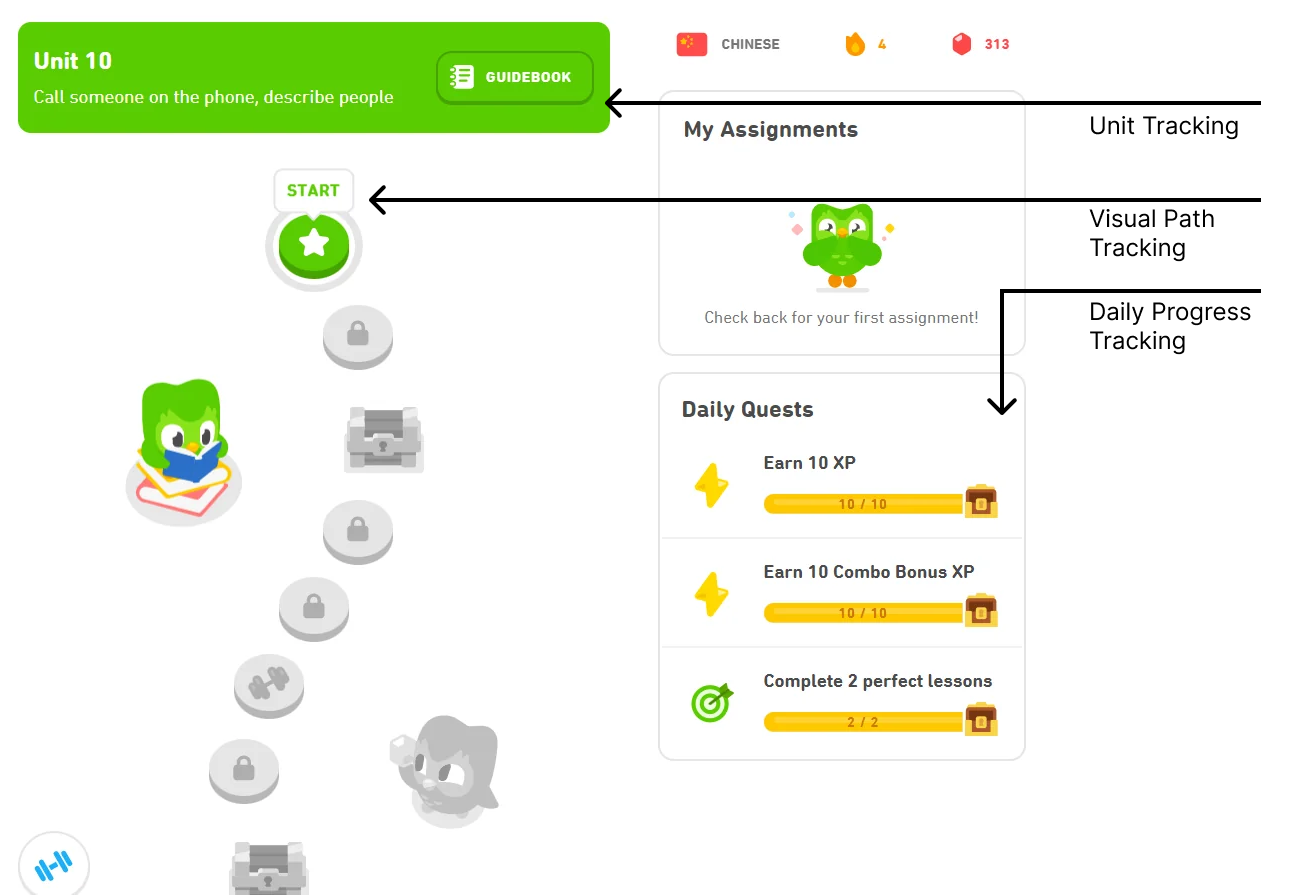
\includegraphics[width=14cm]{Media/DuolingoProgress.png}
 \caption{Various types of Duolingo progress tracking}
 \label{fig:duolingoProgress}
  {\raggedright \small{Source: Duolingo for desktop, 2024}\par}
\end{figure}

However, some research also suggests that while gamification is an excellent engagement boost, especially through social influence, it may not be a guaranteed information retention or personal improvement enhancer, as in more quantitative studies, it was found that gamification only partially outperformed control groups in some areas (\cite{doesItWork}). 
So according to Hamari and Koivisto (2015), while gamification can significantly boost user engagement and participation, improved results for the user are not inherent. 
The pitfalls of the application are the factors of the context that is being gamified as well as the qualities of the users. 
This is further supported by a study by Chernbumroong et al., where people were researched in a virtual reality museum, with either gamified or non-gamified systems in place. 
The gamified version left a much greater impression but negligibly improved information retention (\cite{VR}). 
This suggests that while maintaining the engagement of the user in a learning context can lead to accelerated improvement, it is not guaranteed. 
This is not the case in areas where engagement is key. 
That is particularly relevant in marketing, where social proof, engagement, peer endorsements and attention retention provide excellent marketing opportunities and enhance brand loyalty, recognition and consumer trust through the exposition of products and services.

\subsubsection{Gamification in Marketing}

Gamification has become a valuable tool and has revolutionized marketing strategies by embedding game-thinking scenarios for the audience into brand interactions, thereby fostering greater customer engagement and loyalty (\cite{redefinition}). 
One prominent example of gamification in marketing is the Sephora Beauty Insider program \footnote{https://loyaltylion.com/blog/scale-success-story-sephoras-beauty-insider}. 
The initiative leverages a tiered rewards system where customers earn points for various activities, which can then be exchanged for exclusive rewards. 
This approach not only promotes customer interaction but also encourages repeat purchases by offering tangible incentives. Moreover, gamification has proven effective in boosting brand visibility and recall. 
Robson et al. (2015) found that campaigns incorporating gamified elements tend to receive more shares on social media, thereby amplifying brand reach (\cite{gameon}). 
For instance, McDonald's "Monopoly" promotion engages customers by allowing them to collect game pieces with each purchase \footnote{https://smartico.ai/mcdonalds-uses-gamification-boost-sales-retention/}. 
These pieces can be used to win prizes or traded, thereby increasing both brand exposure and consumer interaction.

Gamification facilitates immersive experiences that enhance customer engagement and loyalty. 
\textcite{doesItWork} observed that gamified features in loyalty programs, such as Starbucks Rewards, lead to improved user satisfaction and retention. 
The program’s use of points and badges motivates frequent interaction, resulting in increased customer spending and stronger brand relationships. 
Regarding badges, a study by \textcite{badges} suggested that badges are a great way to boost a system's usability but also that its engagement tends to decline with time. 
Other challenges are also present according to \textcite{nicholson2015}, that highlight ineffective gamification strategies leading to superficial engagement, and failing to foster long-term loyalty or meaningful behaviour change. 
Additionally, \textcite{gameon} found examples of failed gamification approaches that happened due to no achievements or extrinsic rewards being offered for the user's performance within the intrinsic systems. 
Essentially, a poorly executed campaign that does not resonate with users' intrinsic motivations or provide substantial value may only achieve temporary engagement. 
\begin{figure}[htbp]
  \centering
  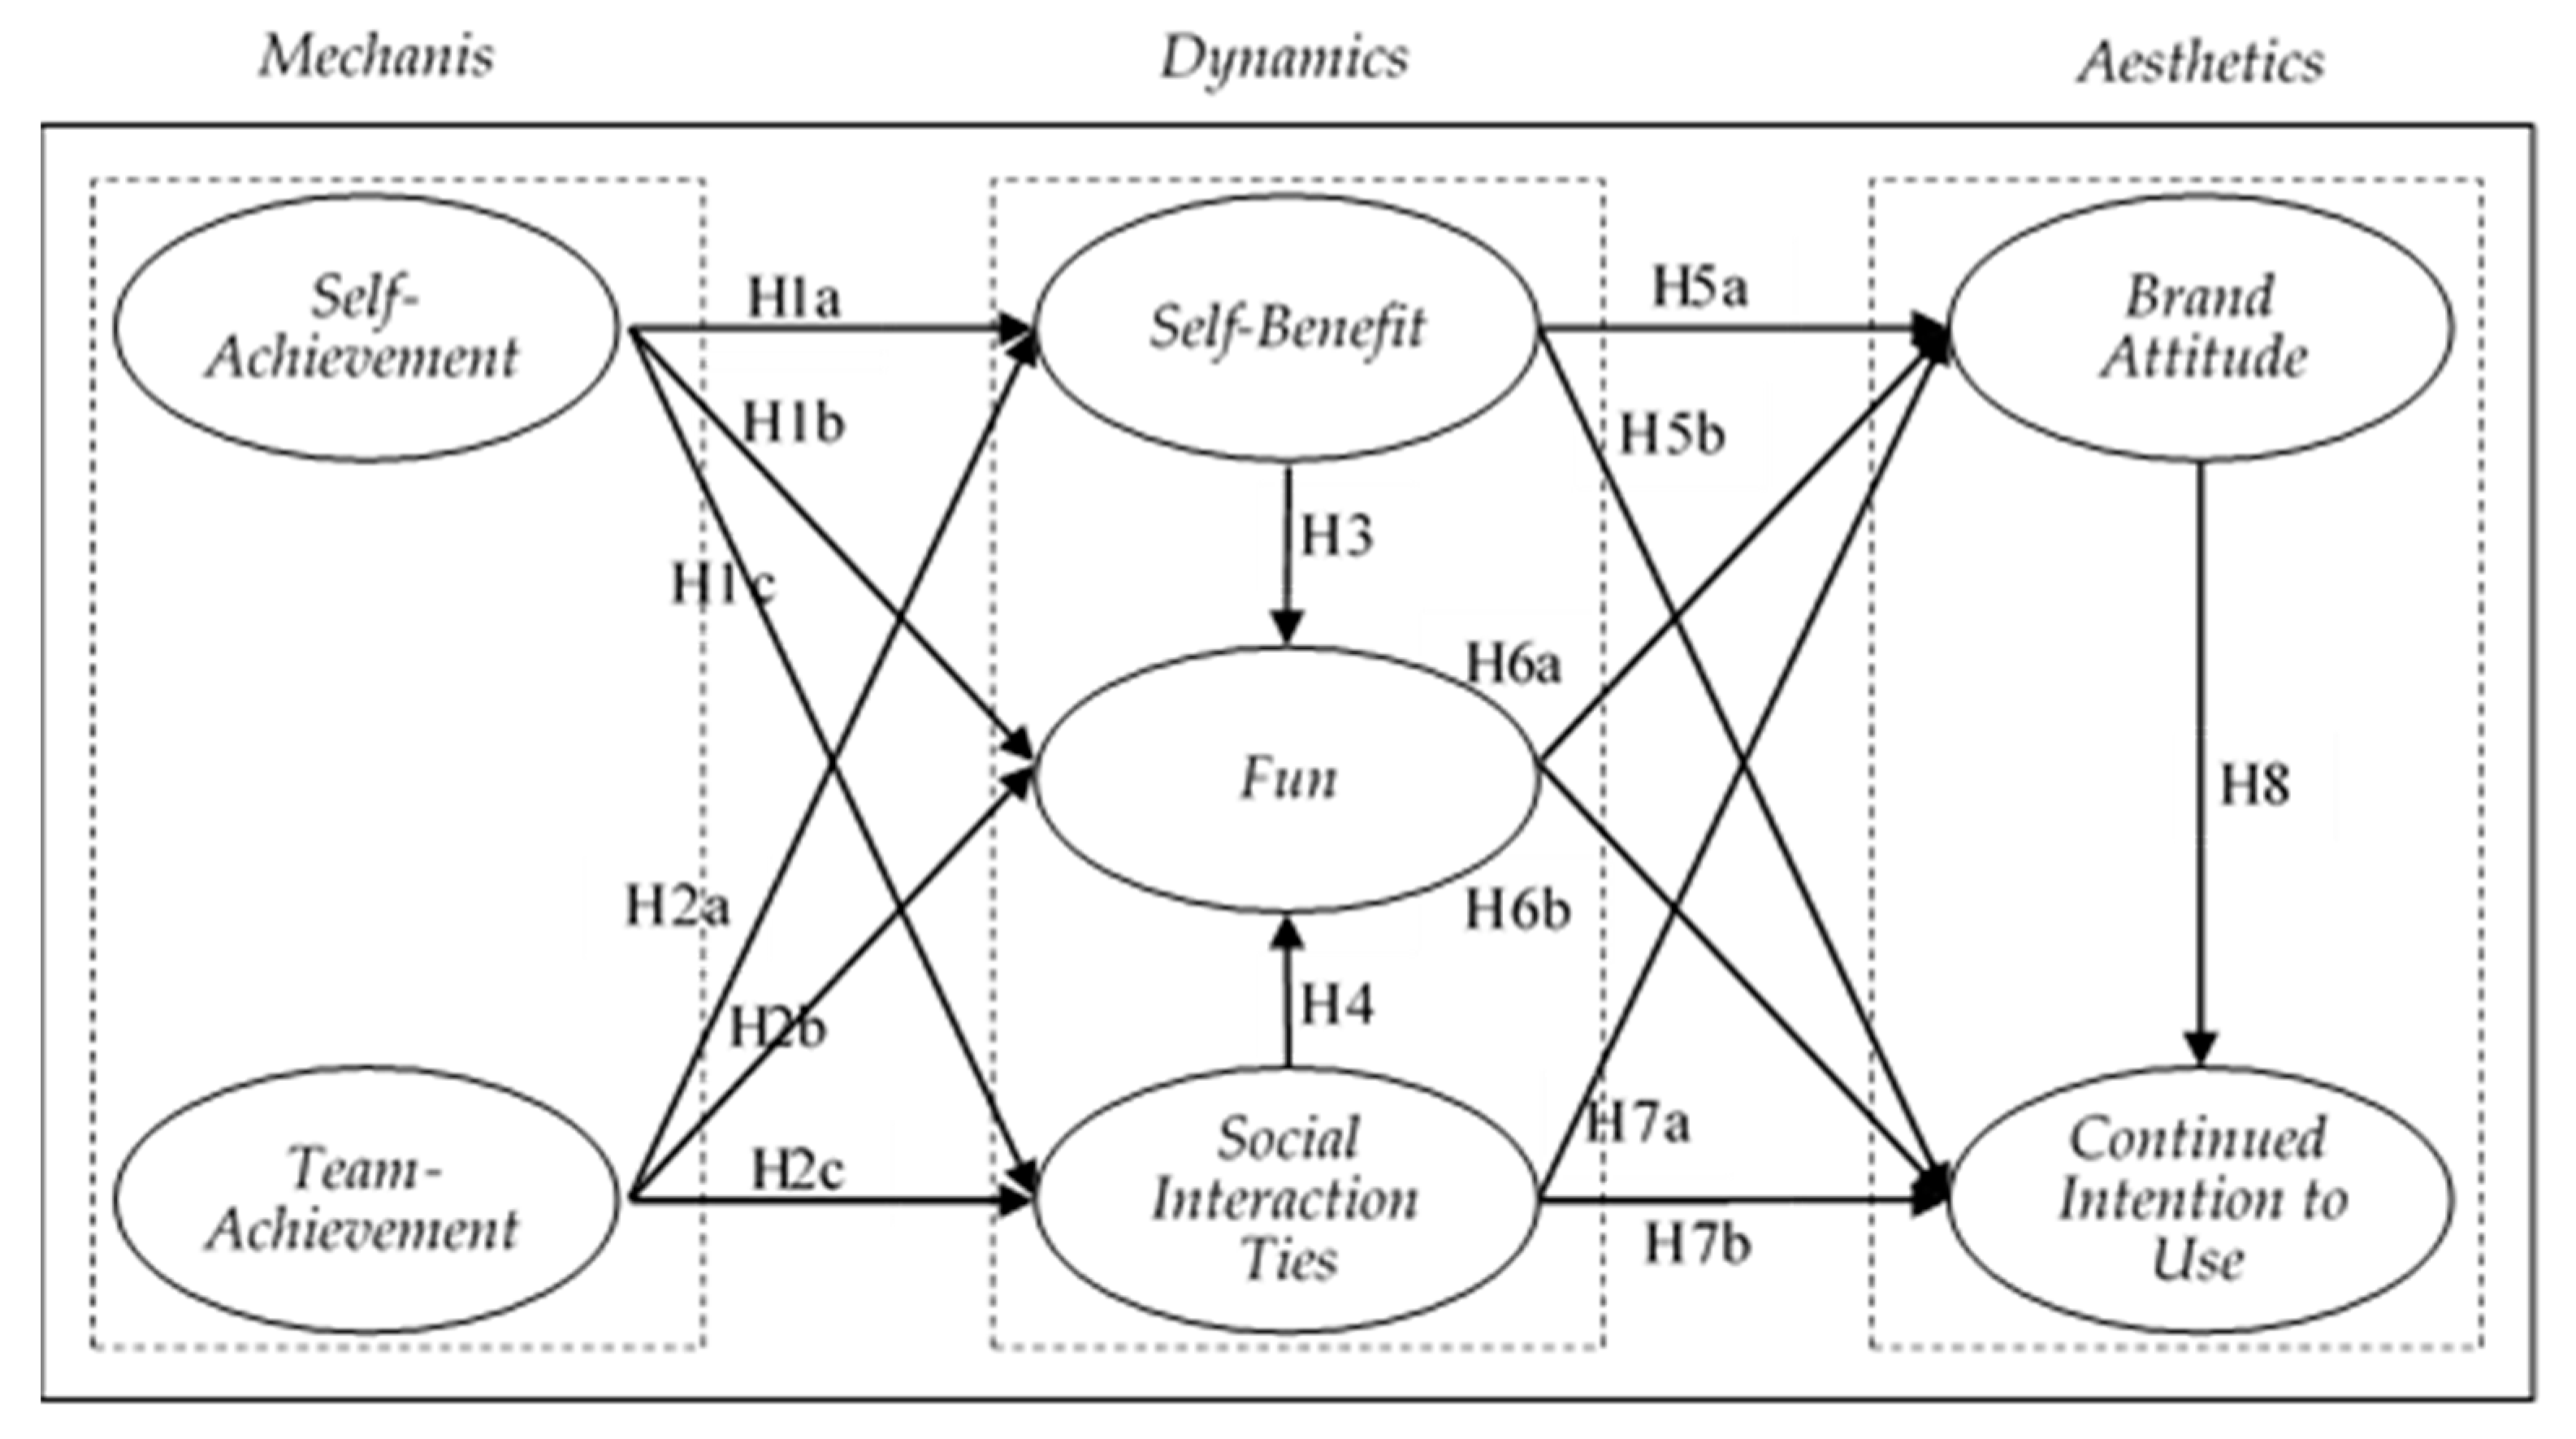
\includegraphics[width=\textwidth]{Media/sustainability2.png}
  \caption{Research model for the \acrshort{mda} framework}
  \label{fig:explainedDataChart}
{\raggedright \small{Source: Hsi-Peng Lu and Hui-Chen Ho, 2020}\par}
\end{figure}
Ensuring that gamified elements are well-aligned with user needs is crucial for sustaining engagement and maintaining a positive brand image.
Evidence from successful programs like Sephora’s Beauty Insider, McDonald's Monopoly and Starbucks Rewards underscore the effectiveness of gamification in marketing.

\subsubsection{Gamification in Web Development}

With web development adapting increasingly more techniques to endlessly growing user engagement, gamification has naturally become one of the pillars of its development. 
Research by \textcite{roleOfMobile} shows that browser games can leverage all of the gamification benefits as well as feature very low entry barriers due to the web's accessibility and popularity. 
Additionally, \textcite{doesItWork} highlight that gamification solutions can substantially enhance software and service user engagement, a principle that applies effectively to browser games.

\textcite{sustainability} explore how gamification affects user engagement in brand applications, demonstrating that gamified strategies can sustain user interaction and strengthen brand connections. 
Games like "Cookie Clicker" employ progression systems and in-game economies to keep players invested and returning over long periods. 
Furthermore, a blog by \textcite{UXdesign} discusses various gamification strategies in digital product design, emphasizing their role in improving user experiences and driving engagement. 
Browser-based educational games like "Prodigy" use rewards and challenges to make learning more engaging, thereby increasing user satisfaction and retention.
Granted, most browser games exist within confined ecosystems like Facebook where they're meant to maintain engagement but solely to keep users terminally online as long as possible with examples like "Farmville".

To better understand the exact elements of gamification to apply in products and services, frameworks were designed to appropriately identify and apply resources to successfully gamify products. 
The most important success factor to achieve gamification of products, systems and services is "fun". 
The \acrshort{mda} framework to achieve "fun" applied by gamification according to research by \textcite{sustainability} consists of the following aspects:

\begin{itemize}
    \item \textbf{Mechanics}:  The rules and systems that guide the gameplay.
    \item \textbf{Dynamics}:  The run-time behaviour of the mechanics, shaped by the players' interactions.
    \item \textbf{Aesthetics}:  The emotional responses or experiences the game evokes in players.
\end{itemize}

This provides a structured way to think about how different elements of game design come together to deliver an engaging experience. 
This is further expanded upon in Figure \ref{fig:explainedDataChart}, which analyzes the relevant aspects of gamification through a study that tests specific applications of each aspect and how they affect each other to achieve marketing goals through a handful of hypotheses. 
An interesting finding within the study was that after measuring the results of the study, team achievements were least efficient in "fun" and end results, which leads to suggest that in spite of the importance of team-building or team-based exercises, team-based elements have to have complementary self-achievement to achieve desired results. 
The study was conducted by gamifying running exercises. 
Notably, the study found that continued usage and brand attitude is more important for newly acquired customers or people who are not yet customers. 
This indicates that gamification is much more efficient in acquiring new customers rather than retaining existing customers. 
Experienced or existing customers may have a different focus and preferences (\cite{sustainability}).

These studies show that gamification, for a handful of purposes, has been in the web development space for a considerable amount of time by now and collectively it is focused on maintaining user engagement and compelling users to stay on relevant platforms and likely acclimate to provider services (\cite{userEngagement}, \cite{gamificationEngagement}).
%
\newpage